\chapter{Introduction}\label{intro}

% TODO: maybe riduce this introduction
In modern CPUs, comprehending program behavior presents significant challenges. It is not 
surprising that software in such environments may occasionally deviate from expected performance 
and behavior. 
This unpredictability may depend on various factors, including interactions with other cores, 
software components, peripherals, real-time events, suboptimal implementations, or a combination 
of these factors.

To tackle this challenge, was developed a less intrusive and efficient technique to performance 
debug: tracing.
The RISC-V consortium developed the open-source RISC-V ISA and also connected non-ISA 
specification, among these is present the \textit{RISC-V Efficient Trace (E-Trace)}. This 
specification is a standardized processor trace method that defines an efficient compressed 
branch trace algorithm, input port specifications, and trace output packet formats. 

To implement the E-Trace specification, the Trace Encoder (TE) was developed.
To get more detail about branch tracing and the trace encoder design refer to the associated 
documentation.

Now, the TE produces the output packets as defined in the specs, but there's a problem: right now 
it is not possible to read the output produced by the TE outside simulation. To overcome this 
issue the RISC-V consortium also developed the \textit{Unformatted Trace \& Diagnostic Data 
Packet Encapsulation for RISC-V}, that describes a module that transforms the tracing data into standard 
packets sendable off-chip. 

The specification does not specify what are the inputs and the outputs: for our specific usecase 
the input is obviously the TE output. The output is not specified either, but the protocol more 
practical for our usecase is the \textit{ARM Trace Bus} (ATB).

This protocol was chosen due to the fact that is design to transport tracing data and that it can 
be easily converted to other more capable protocol such as AXI. From AXI it can be converted to 
PCIe and data can be sent to the debug device.

The architecture chosen is designed to be easily adapted to other communication protocols on the output.

\begin{figure}[H]
    \centering
    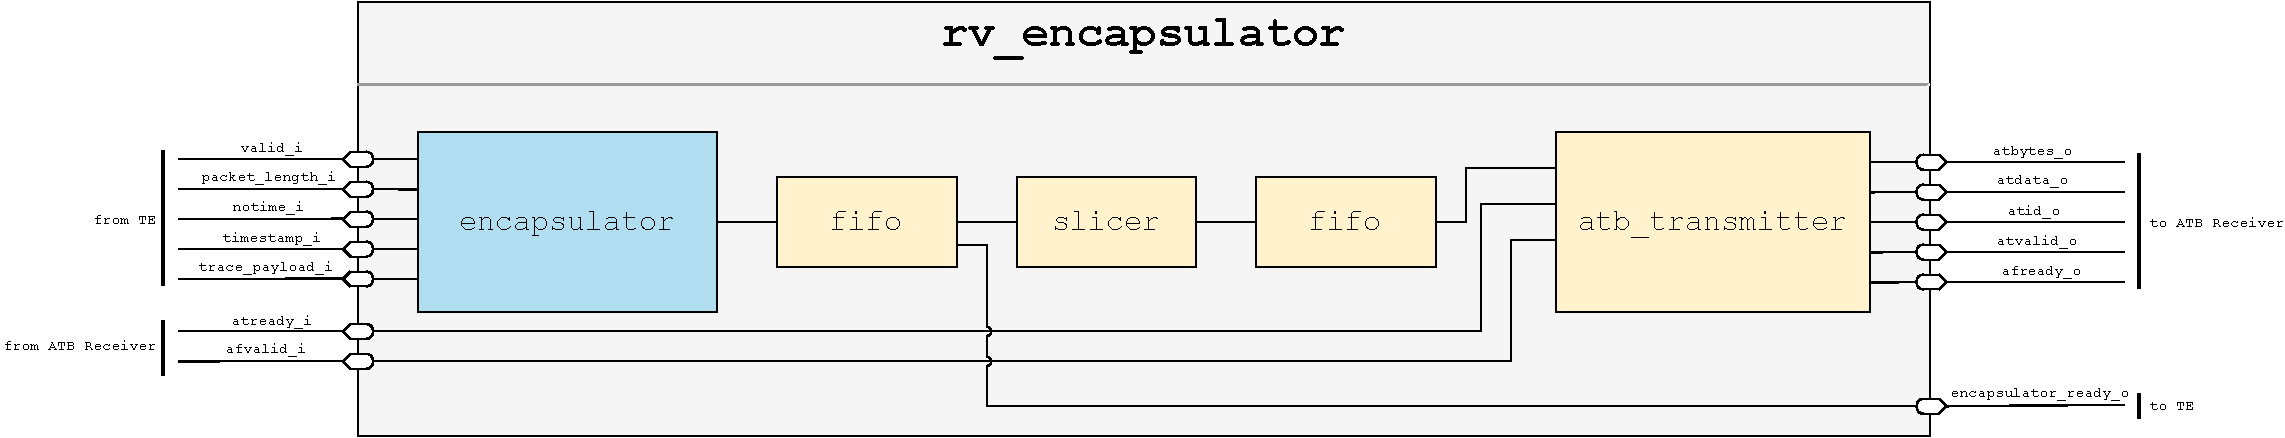
\includegraphics[width=1\textwidth]{img/rv_encapsulator.pdf}
    \caption{Top level module internal architecture}
    \label{fig:rv_encapsulator_architecture}
\end{figure}